\section{Anatomy of a CBIR System}\label{sec:anatomy}

The inner workings of most CBIR systems can best be examined by looking at the
processing pipeline each query has to go through. The coarse sequence of
computational steps is almost the same in all such systems (Figure
\ref{fig:cbir_coarse_structure}):

\begin{enumerate}
    \item Acquire the image.
    \item Extract the signature using a feature extraction algorithm.
    \item Compare the signature to a database containing the signatures of the
        images to search within.
    \item Rank the images by similarity using the comparison results.
\end{enumerate}

\begin{figure}[h]
    \centering
    \subfloat[Local features]{%
        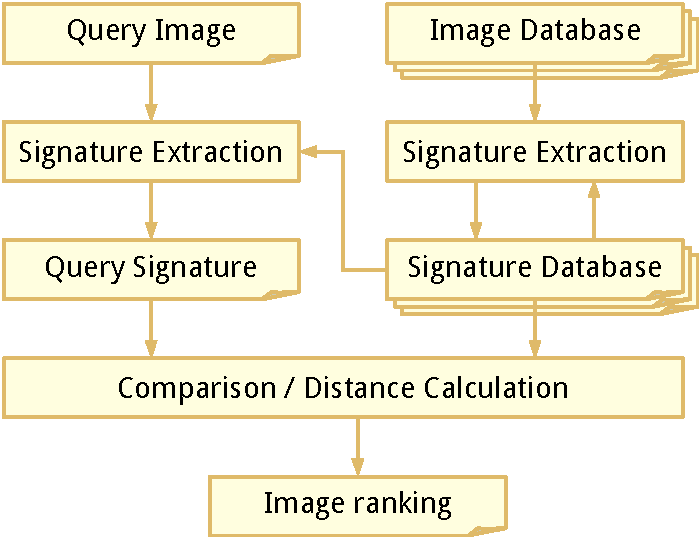
\includegraphics[width=0.45\textwidth]{cbir_anatomy_query_local_cropped}%
        \label{fig:cbir_coarse_structure_local}%
    }
    \quad
    \subfloat[Global features]{%
        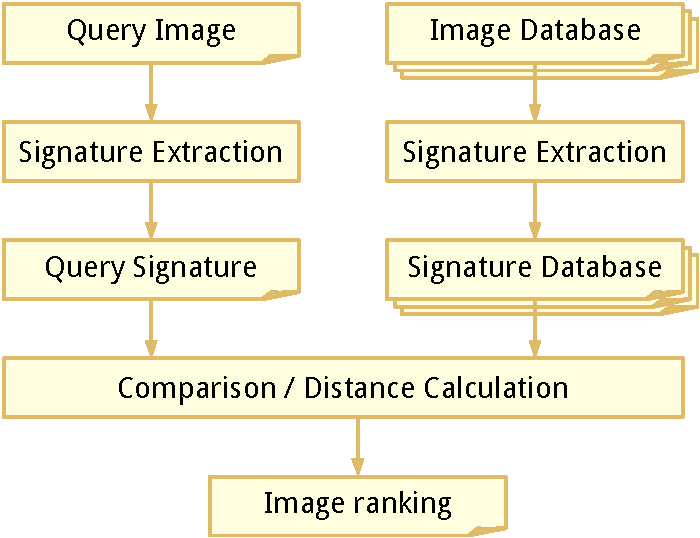
\includegraphics[width=0.45\textwidth]{cbir_anatomy_query_cropped}%
        \label{fig:cbir_coarse_structure_global}%
    }
    \caption[Coarse structure of a CBIR system]{
        The processing pipeline for CBIR using both local and global features
        is very similar. The main difference is in the signature extraction
        step, in which local features are selected, weighted and/or compressed
        depending on the results of the signature extraction of the other
        images in the database.
    }
    \label{fig:cbir_coarse_structure}
\end{figure}

\subsection{Image Acquisition}\label{sec:anatomy_image_acquisition}

The format in which the images are available to the system determines the
maximum amount of information available to subsequent analysis steps.

A significant part of the preprocessing usually done after acquisition depends
on the broadness of the image domain. The concept of the domain encompasses and
describes the variability of many possible image parameters like illumination
or composition and is therefore closely related to the sensory gap described
above. The narrower the image domain is, the more assumptions the system can
make about image from that domain. By their very nature, the domain of sketch
based image retrieval systems is usually very broad. It contains the sketches
create by the user to query the database as well as the images in the database
itself, which can be of a completely different nature, e.g.\ photos or
paintings.

Another factor usually is the accepted input format of the feature extraction
algorithm. Many algorithms like SIFT \autocite{lowe_object_1999} or SURF
\autocite{bay_speeded-up_2008} are defined for single-channel data, but some
have been specifically developed to operate on multi-channel images, like cSIFT
\autocite{abdel-hakim_csift:_2006} and \autocite{yang_robust_2008}.

\subsection{Signature Extraction}\label{sec:anatomy_signature_extraction}

The signature of an image is its representation in the following comparison
step. Therefore it should describe the image using its most discriminatory
features compared to all other images in the database. Due to the effects of
the \emph{sensory gap} discussed above, there is, at the moment, no definitive
way to determine the discriminatory power of features in general, even though
knowledge about the image domain can guide the descisions.

The signature composition depends on both, the kind of features extracted from
the image and the way these features are encoded. Over the last two decades, a
wide variety of feature descriptors have been published, which mostly focus on
specific types of features. Some techniques use color histograms
\autocite{utenpattanant_color_2006}, while others
\autocite{stricker_color_1996} \autocite{deng_efficient_2001}
\autocite{lee_spatial_2003} include spatial relations between colors in a
region. Many descriptors attempt to capture
texture characteristics, such as \autocite{schaffalitzky_viewpoint_2001} and ...
SHAPE here (sift).
Several publications combine feature types to arrive at a more comprehensive
descriptor. Oliva and Torralba \autocite{oliva_modeling_2001} capture various
scene "roperties like "roughness" and "openness". more examples here.

\begin{figure}[h]
    \centering
        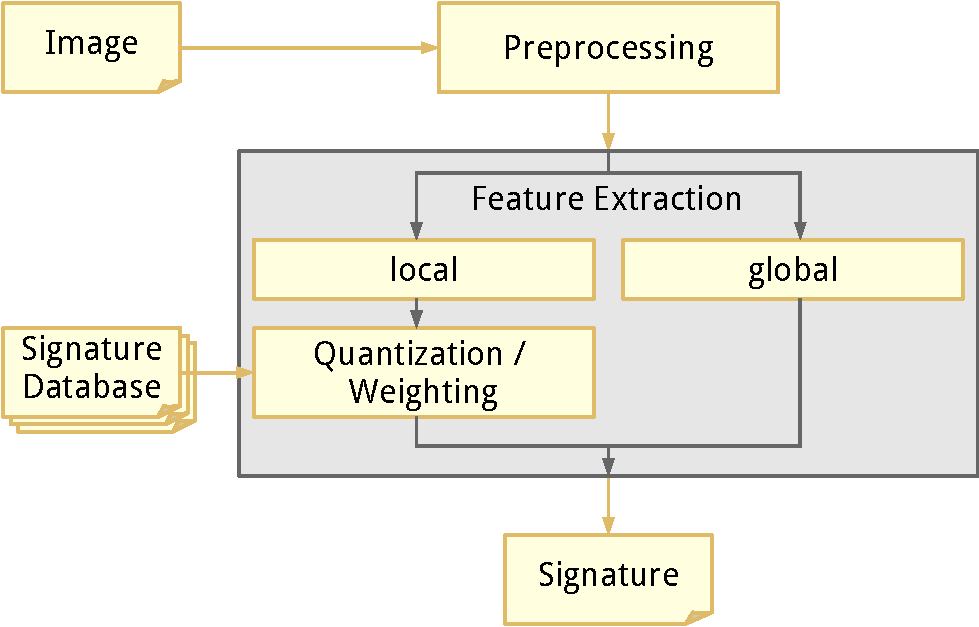
\includegraphics[width=0.8\textwidth]{cbir_anatomy_signature_extraction_cropped}
    \caption{Signature extraction in CBIR systems}
    \label{fig:cbir_signature_extraction}
\end{figure}

\subsection{Comparison and Ranking}\label{sec:anatomy_ranking}

TBD
